\subsection{Proceso Interno 02: Inicializar Población}

\subsubsection{Objetivo del Proceso}
El propósito principal de la actividad \textbf{``Inicializar Población''} es generar un conjunto inicial de $N$ individuos que sirvan como punto de partida para el algoritmo bioinspirado del proyecto \textit{``Modelo para representar comportamientos gravitacionales con dos cuerpos''}. Cada individuo representa un conjunto completo de parámetros a optimizar (ej\ masas de cuerpos), generados dentro de los rangos válidos especificados en la configuración.

\subsubsection{Entradas Principales}
\begin{itemize}
    \item \textbf{ConfigurationData}: Estructura con:
    \begin{itemize}
        \item Tamaño de población $N \in \mathbb{N}$
        \item Rangos por parámetro: $[\min, \max]$ (ej.\ $[\texttt{masa}_{1,~\min}, \texttt{masa}_{1,~\max}]$)
    \end{itemize}
    \item \textit{Nota}: Restricciones funcionales se manejarán posteriormente
\end{itemize}
\subsubsection{Sub-pasos Secuenciales}
Este apartado es proporcionado para profundizar y describir de forma textual cada paso contenido dentro del diagrama del proceso descrito en la figura~\ref{fig:process_diagram02}
\subsubsection*{1. Leer Configuración Relevante}
\begin{itemize}
    \item Extraer de \texttt{ConfigurationData}:
    \begin{itemize}
        \item $N$
        \item Lista de parámetros a optimizar
        \item Rangos asociados
    \end{itemize}
    \item Verificar coherencia: $\forall \text{parámetro}, \min < \max$
\end{itemize}

\subsubsection*{2. Inicializar Contenedor de Población}
\begin{itemize}
    \item Crear estructura vacía (lista/array) para $N$ individuos
\end{itemize}

\subsubsection*{3. Iniciar Bucle de Creación de Población}
\begin{enumerate}[label= (\alph*)]
    \item Inicializar contador $i = 0$
    \item \textbf{Mientras} $i < N$:
    \begin{itemize}
        \item Generar parámetros candidatos:
        \begin{itemize}
            \item $\forall$ parámetro: valor aleatorio $\in [\text{min}, \text{max}]$
        \end{itemize}
        \item Agregar candidato a la población
        \item $i \leftarrow i + 1$
    \end{itemize}
\end{enumerate}

\subsubsection*{4. Verificar Población Generada}
\begin{itemize}
    \item Confirmar $|\text{población}| = N$
    \item \textit{(Opcional)} Analizar distribución/diversidad
\end{itemize}

\subsubsection*{5. Finalizar y Devolver Población Inicial}
\begin{itemize}
    \item Retornar estructura poblada lista para optimización
\end{itemize}

\subsubsection{Lógica Interna y Decisiones}
\begin{itemize}
    \item \textbf{Control del bucle}: Garantiza generación exacta de $N$ individuos
    \item \textbf{Generación en rangos}:
    \begin{itemize}
        \item Aleatorización restringida por $[\min, \max]$
        \item Elimina necesidad de validación posterior
    \end{itemize}
    \item \textbf{Verificación crítica}:
    \begin{itemize}
        \item Precondición: $\min < \max$ $\forall$ parámetro
    \end{itemize}
    \item \textbf{Diversidad opcional}:
    \begin{itemize}
        \item Métricas estadísticas no requeridas en flujo principal
    \end{itemize}
\end{itemize}

\subsubsection{Manejo de Datos Específico}
\begin{itemize}
    \item \textbf{Entrada}: \texttt{ConfigurationData}
    \item \textbf{Intermedios}:
    \begin{itemize}
        \item Valores aleatorios $\in$ rangos
        \item Estructuras temporales por individuo
    \end{itemize}
    \item \textbf{Salida}: Lista/array de $N$ individuos
\end{itemize}

\subsubsection{Salidas Principales}
\begin{itemize}
    \item \textbf{Población inicial}:
    \begin{itemize}
        \item $N$ individuos con parámetros $\in$ rangos
        \item Entrada para evaluación de $LE$
    \end{itemize}
\end{itemize}

\subsubsection{Interacciones Internas}
\begin{itemize}
    \item \textbf{Con \texttt{ConfigurationData}}: Lectura de parámetros
    \item \textbf{Con generador aleatorio}: Producción de valores válidos
    \item \textbf{Con estructura de población}: Almacenamiento y gestión
\end{itemize}
\newpage
\subsubsection{Diagrama del Proceso}
\begin{figure}[H]
    \centering
    \adjustbox{max width=\textwidth, max height=0.9\textheight}{%
        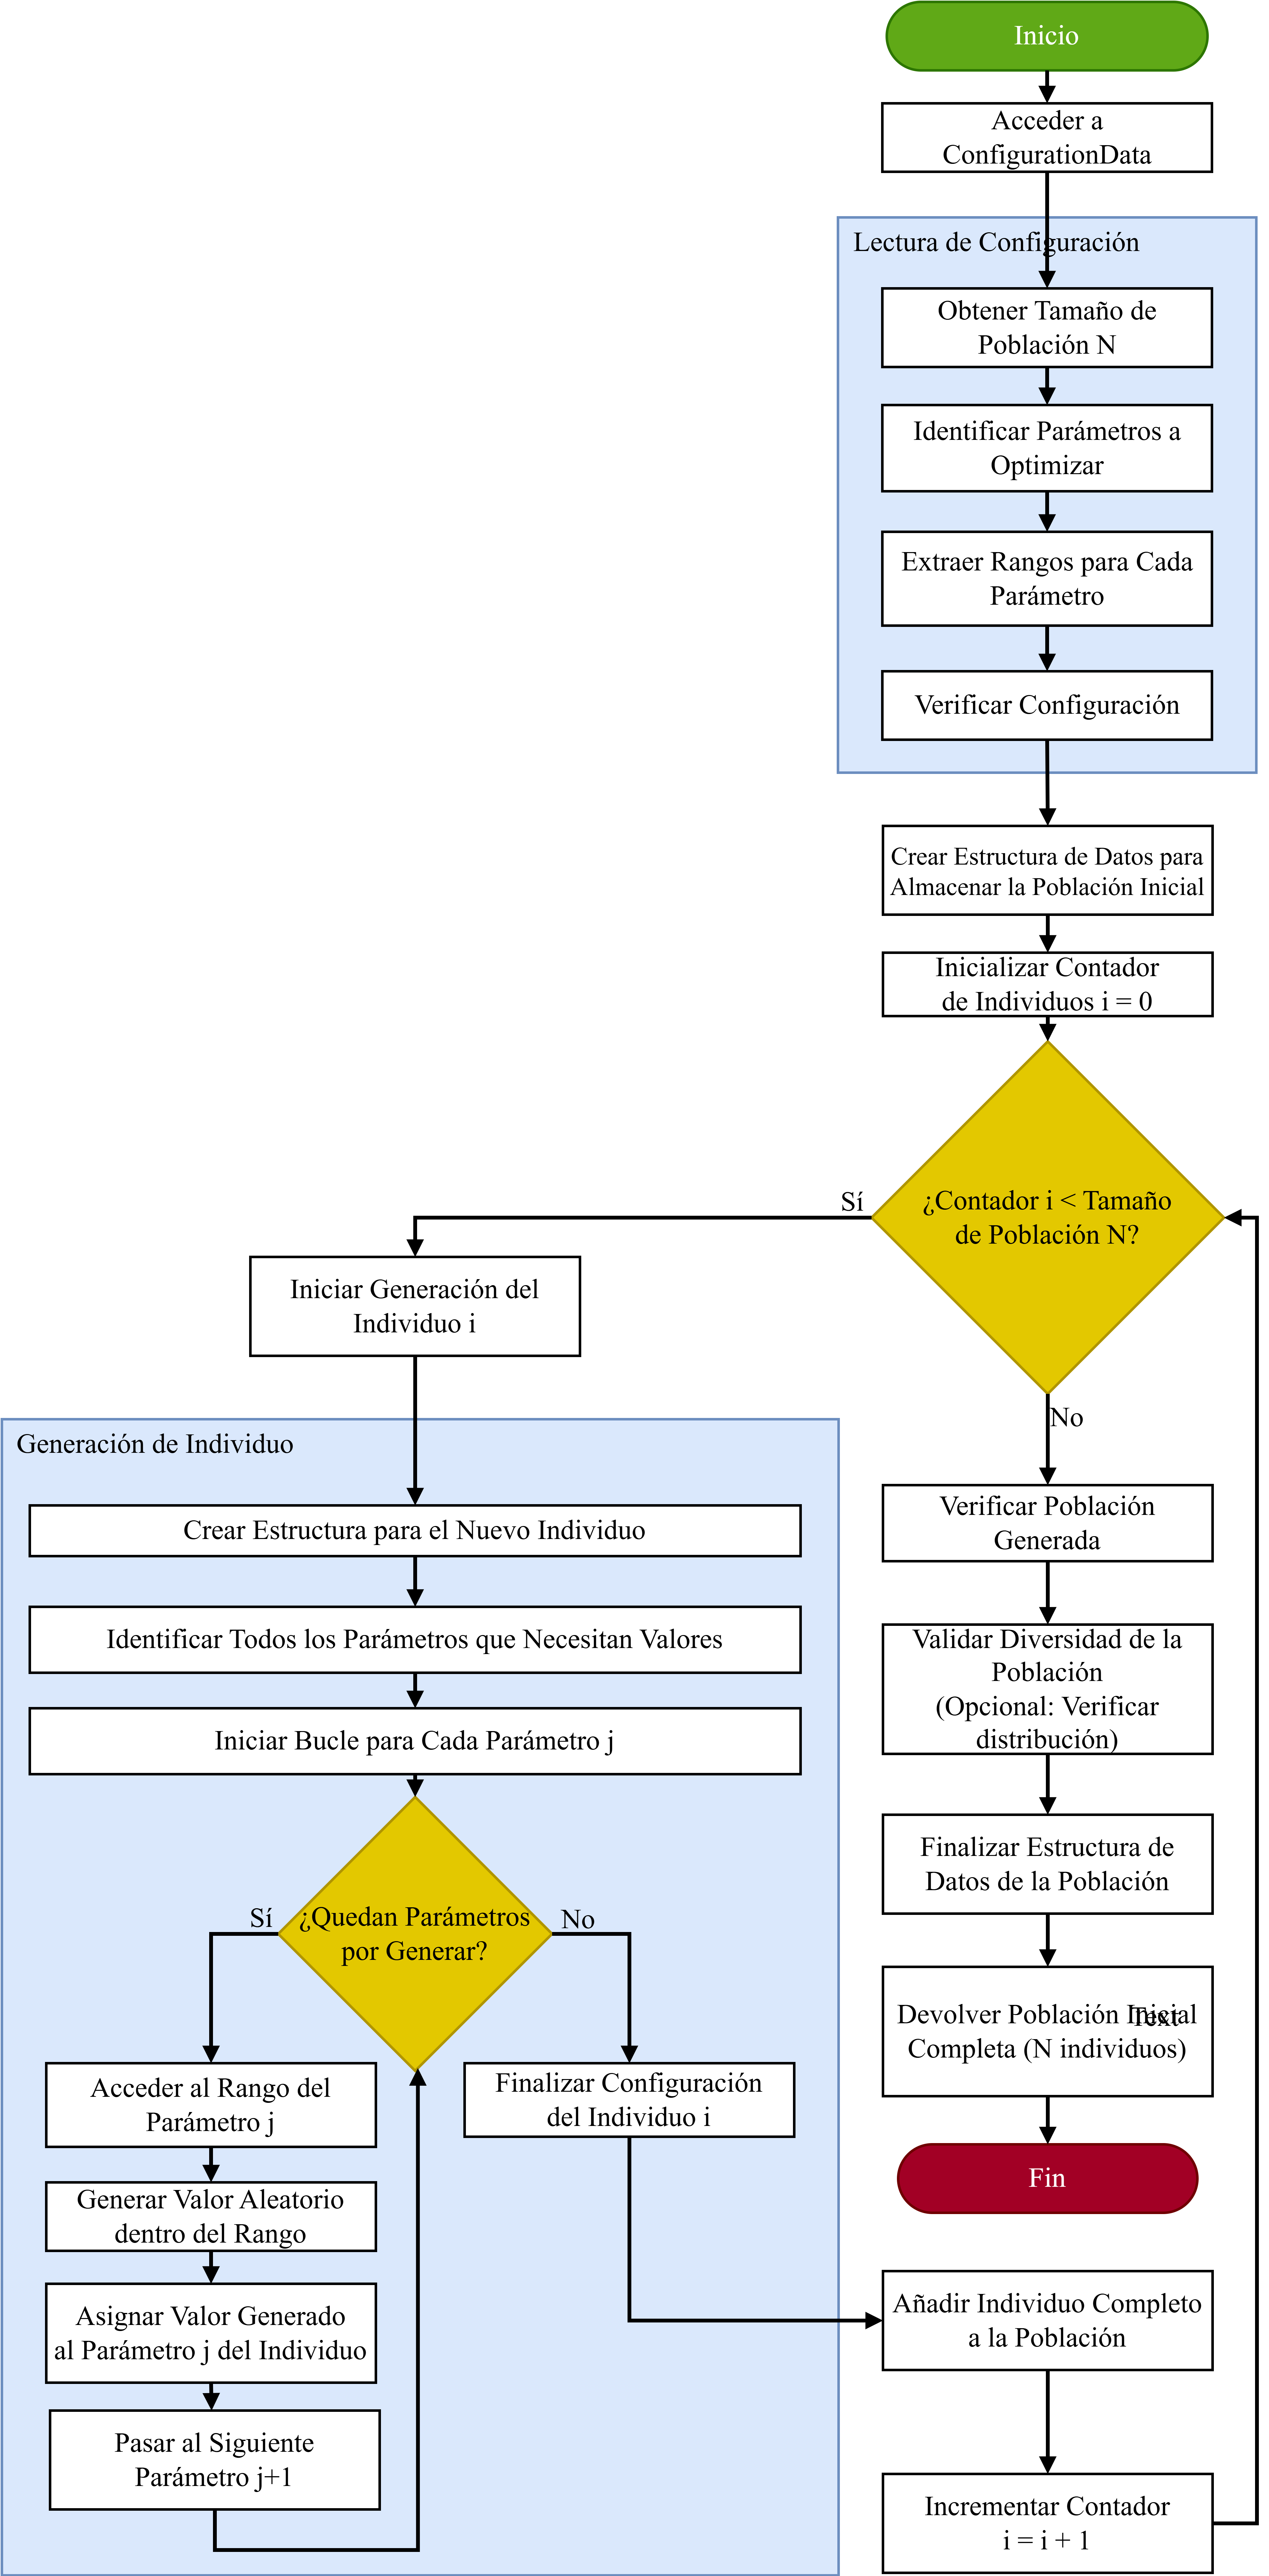
\includegraphics{img/Analisis/DiagramaProcesos/DiagramaProceso02_InicializarPoblacion.png}
    }
        \caption{Diagrama de Proceso Interno 02: Inicializar Población}%
    \label{fig:process_diagram02}
\end{figure}
\newpage